\section{Ladeelektronik}
Nach längerer Überlegung wurde entschieden kein Batteriemanagement selbst zu entwerfen, sondern ein Ladegerät und ein Schaltnetzteil zuzukaufen. \\

\textbf{Eine Anleitung für den Ladevorgang findet man im \autoref{sec: bilderanleitung_laden}.}

% \subsection{Akkumulatoren}
% Als Akkumulatoren wurden 2x vier, TopFuel LiPo 35C Power-X 7500mAh 7s in Serie geschaltet, siehe \autoref{sec:Akkus}. \\

\subsection{Ladegerät}
Verwendet wird das Ladegerät \glqq iSDT SMART Dup Ladegerät P30 - 1500W, 30A\grqq. Das Ladegerät ist ein 2-Kanalladegerät, das heißt, 
dass beide Akku-Stränge gleichzeitig geladen werden können. 
Das P30 kann mit dem Programm \glqq Dual Task\grqq beide Kanäle mit dem selben Programm laufen lassen. Somit gibt man die Ladeparameter nur einmal ein. \\
Der maximale Ladestrom beträgt 30$\mathrm{A}$ pro Strang. \\
Weitere Infos sind unter \href{https://www.modell-hubschrauber.at/Ladegeraete-Netzteile-Ladekabel-und-Zubehoer/Ladegeraete/Ladegeraete-12Volt/iSDT-SMART-Dup-Ladegeraet-P30-1500W-30A-8S-Lipo::43075.html}{Link zur Website} 
zu finden. 

\begin{figure}[H]
    \centering
    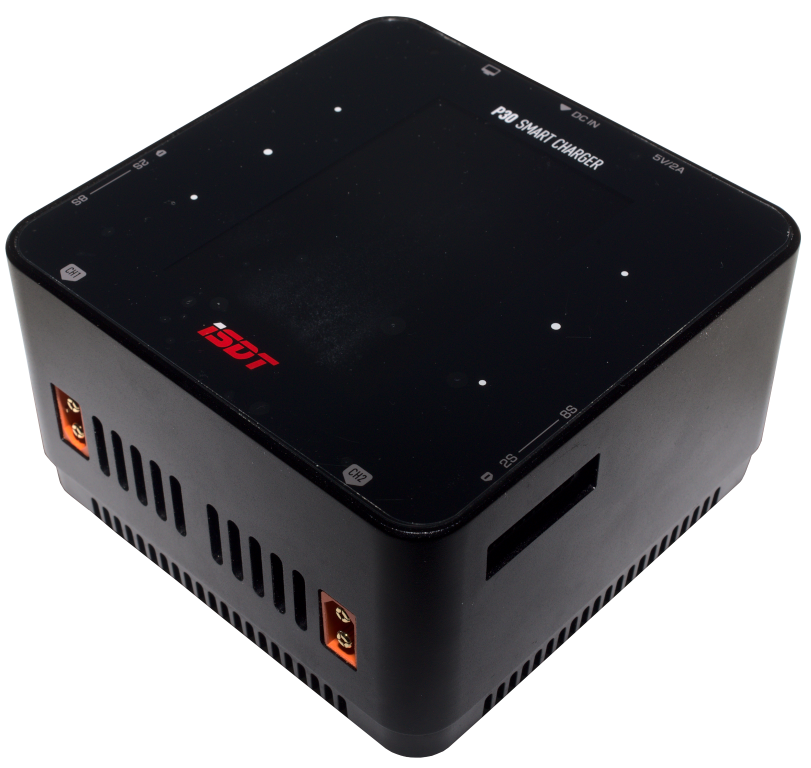
\includegraphics[width=0.7\textwidth]{Fotos/SP30_DSC_8784.png}
    \captionof{figure}{Ladegerät}    
\end{figure}

\subsection{Schaltnetzteil}
Die Wahl fiel auf das, zum Ladegerät empfohlene, \glqq iSDT SP3060 SMART POWER Schaltnetzteil\grqq.
Das Schaltnetzteil ist gegen Überlast, Überspannung, Überhitzung und Kurzschluss geschützt. 

\begin{minipage}{13cm}
    \centering
    \includegraphics[width=0.65\textwidth]{Fotos/SP3060.png}
    \captionof{figure}{Schaltnetzteil}   
\end{minipage}

\newpage

